% Reporte técnico, proyecto 3 de TinyML 2026.
% Las cifras salen de resultados/, generadas por Proyecto_3.py y compilar_sketches.py.
% Lo marcado con \pendiente{} depende de la sesión con la placa o de datos del equipo.
% Paquetes que usa el cuerpo, por si se cambia de plantilla: graphicx, booktabs, xcolor,
% tikz con las bibliotecas arrows.meta y positioning, caption y hyperref.
% Las figuras van en figuras/ y son copias de resultados/.
\documentclass[11pt,a4paper]{article}
\usepackage[T1]{fontenc}
\usepackage[utf8]{inputenc}
\usepackage[spanish,es-noshorthands,es-tabla,es-nodecimaldot]{babel}
\usepackage{lmodern}
\usepackage[margin=2.4cm]{geometry}
\usepackage{graphicx}
\usepackage{booktabs}
\usepackage{xcolor}
\usepackage{tikz}
\usetikzlibrary{arrows.meta,positioning}
\usepackage{caption}
\usepackage[hidelinks]{hyperref}

\graphicspath{{figuras/}}
\newcommand{\pendiente}[1]{\textcolor{red}{\textbf{[PENDIENTE: #1]}}}
\captionsetup{font=small,labelfont=bf}

\title{Reconocimiento de actividad física con TinyML\\[2pt]
\large Arduino Nano 33 BLE Sense: adquisición, entrenamiento, cuantización INT8 e inferencia en el microcontrolador}
\author{\pendiente{nombres de los integrantes}}
\date{TinyML 2026, proyecto 3}

\begin{document}
\maketitle

\begin{abstract}
Se construyó un clasificador de cinco actividades que corre por completo en un Arduino Nano 33 BLE Sense a partir de su unidad de medición inercial. Las actividades son reposo, caminar, correr, subir escaleras y bajar escaleras. El conjunto de datos tiene una sesión de 60~s por actividad de cada una de tres personas, muestreada a 50~Hz. Las señales se dividen en ventanas de 2~s. A cada ventana se le resta su media, lo que elimina la gravedad y con ella la orientación con que se colocó la placa. Después se normaliza cada canal y una red convolucional 1D de 8\,165 parámetros clasifica la ventana. Con evaluación dejando una persona fuera, el modelo con solo el acelerómetro alcanzó una exactitud de 0.831 y el de acelerómetro más giróscopo alcanzó 0.768. La cuantización INT8 redujo el modelo de 39\,156 a 17\,728 bytes sin cambiar la exactitud, que fue de 0.832. Sus predicciones coinciden con las del modelo FP32 en el 98.6\,\% de las ventanas. Los cuatro programas para la placa compilan y caben con holgura, con 193 a 216~KB de Flash y 84.7~KB de RAM estática. La latencia y la memoria usada en la placa están \pendiente{sesión con la placa}.
\end{abstract}

\section{Cuestionario previo}

\paragraph{1. ¿Qué es una IMU y qué magnitudes mide?}
Una unidad de medición inercial combina sensores que miden el movimiento de un cuerpo sin una referencia externa. Suele incluir un acelerómetro de tres ejes, que mide la fuerza específica en $g$, es decir, la aceleración lineal más la reacción a la gravedad. También incluye un giróscopo de tres ejes, que mide la velocidad angular en grados/s, y a menudo un magnetómetro, que mide el campo magnético. La Nano 33 BLE Sense Rev1 usa el LSM9DS1, que es de nueve ejes. En este proyecto se usan los seis ejes inerciales.

\paragraph{2. ¿Cuál es la diferencia entre un acelerómetro y un giróscopo?}
El acelerómetro mide la aceleración a lo largo de cada eje, incluida la gravedad. En reposo indica la inclinación de la placa respecto a la vertical, pero no el giro alrededor de ella. El giróscopo mide qué tan rápido gira la placa alrededor de cada eje y no percibe la gravedad. Al integrarlo se obtienen cambios de orientación, pero con deriva por su sesgo. En los datos, el giróscopo en reposo marca unos $-2.2$~grados/s en el eje $y$ en las tres personas, y ese valor es el sesgo del sensor.

\paragraph{3. ¿Qué información proporciona cada eje del acelerómetro?}
Cada eje da la proyección de la fuerza específica sobre ese eje de la placa. En reposo es la componente de la gravedad, de donde sale la inclinación. En movimiento se suma la aceleración dinámica en esa dirección. En los datos el eje $y$ quedó casi vertical, con $a_y$ entre 0.86 y 0.96~$g$ en reposo. Por eso $a_y$ lleva el rebote vertical de cada paso, mientras que $a_x$ y $a_z$ llevan el balanceo horizontal.

\paragraph{4. ¿Por qué es importante una frecuencia de muestreo constante?}
El modelo aprende patrones medidos en número de muestras, no en segundos. Si la frecuencia cambia, el mismo paso aparece estirado o comprimido y la ventana cubre otra duración. En la captura, el intervalo entre muestras estuvo entre 19\,910 y 20\,095~$\mu$s, con una desviación máxima de 26~$\mu$s por sesión. En la placa se muestrea con un temporizador de 20~ms basado en \texttt{micros()}, y el programa cuenta las lecturas que llegan tarde.

\paragraph{5. ¿Qué es una ventana temporal y cómo influye su duración?}
Es un tramo de $N$ muestras consecutivas que se clasifica como una unidad. Debe contener al menos uno o dos ciclos del movimiento, y un paso dura del orden de 0.3 a 1~s según la actividad y la persona. Una ventana más larga da más contexto y estabilidad, pero aumenta la latencia de la decisión y mezcla actividades en las transiciones. Una ventana más corta reacciona antes, pero con menos información. Se usaron ventanas de 2~s, es decir, de 100 muestras, como sugiere el enunciado.

\paragraph{6. ¿Qué ventajas y desventajas tienen las ventanas superpuestas?}
La primera ventaja es que se obtienen más ejemplos de entrenamiento con los mismos datos. La segunda es que las predicciones son más frecuentes. Aquí, con 75\,\% de traslape, hay una predicción cada 0.5~s. La tercera es que se pueden promediar predicciones consecutivas. La desventaja principal es que las ventanas vecinas comparten muestras y no son independientes. Si unas caen en entrenamiento y otras en prueba, la métrica sale optimista, y por eso la evaluación separa por persona. Además, el costo de cómputo se multiplica, pues hay 4 inferencias por cada 2~s de señal.

\paragraph{7. ¿Por qué es necesario normalizar las señales?}
Los canales tienen escalas muy distintas. En los datos la aceleración llega a $\pm4~g$ y la velocidad angular a unos $\pm230$~grados/s. Sin normalizar, los canales grandes dominan el gradiente y la optimización queda mal condicionada. En TinyML hay una razón más. El tensor de entrada INT8 comparte una sola escala, así que sin normalizar el giróscopo ocuparía todo el rango y la aceleración se cuantizaría con muy pocos niveles. Las estadísticas se calculan solo con los datos de entrenamiento y se guardan en el programa de la placa.

\paragraph{8. ¿Qué problemas hay si los datos provienen de una sola persona?}
El modelo aprende la manera de moverse de esa persona, como su cadencia y la amplitud de sus pasos, y también la forma particular en que llevó el sensor. Por eso no generaliza a otras personas. Además, evaluarlo con la misma persona da cifras optimistas. Los datos lo muestran incluso con tres personas. Sin restar la media de cada ventana, la exactitud con una persona no vista fue de 0.27 y el reposo de esa persona nunca se reconoció. El modelo había memorizado la inclinación con que cada persona de entrenamiento llevó la placa, como se detalla en la sección~\ref{sec:prepro}.

\paragraph{9. ¿En qué consiste la cuantización INT8 y qué ventajas ofrece?}
La cuantización INT8 representa pesos y activaciones con enteros de 8 bits mediante la transformación afín $r = s\,(q - z)$, donde $s$ es la escala y $z$ el punto cero. Los sesgos quedan en enteros de 32 bits y las escalas de las activaciones se calibran con un conjunto representativo. Reduce cuatro veces la memoria de los pesos, y en este proyecto el archivo del modelo bajó 55\,\%. También permite aritmética entera y kernels con instrucciones SIMD, como los de CMSIS-NN en el Cortex-M4, y suele reducir la energía. El costo es un error de redondeo, que aquí no cambió la exactitud. No garantiza menor latencia. En el proyecto~1, en esta misma placa, INT8 fue más lento que FP32 en una red densa pequeña, así que la latencia debe medirse.

\paragraph{10. ¿Qué métricas evalúan la calidad y la eficiencia de un modelo TinyML?}
Para la calidad se usan la exactitud, la precisión, la exhaustividad o \emph{recall}, el F1 por clase y su promedio macro, y la matriz de confusión. Todas deben medirse con personas que el modelo no vio. Para la eficiencia se usan el tamaño del modelo en bytes y en parámetros, las operaciones por inferencia o MAC, la Flash y la RAM estática del programa, la memoria usada de la \emph{tensor arena} y la latencia por inferencia con su mínimo, máximo, promedio y desviación. Si se puede medir, también se reporta la energía por inferencia. Para la cuantización se reporta además qué tanto coinciden las predicciones FP32 e INT8.

\section{Conjunto de datos}\label{sec:datos}

\paragraph{Adquisición.}
Se usó la Arduino Nano 33 BLE Sense Rev1 con la biblioteca \texttt{Arduino\_LSM9DS1} 1.1.1. Esta biblioteca configura el acelerómetro a $\pm4~g$ y el giróscopo a $\pm2000$~grados/s, ambos a 119~Hz. El programa de captura los leyó a 50~Hz y guardó el tiempo de cada lectura en microsegundos. Tres personas realizaron cada actividad durante 60~s en una sesión continua. La placa se colocó \pendiente{posición y forma de sujeción de la placa, agregar foto}. En los datos, el eje $y$ de la placa apuntó hacia arriba en las tres personas.

\paragraph{Contenido.}
Son 45\,000 muestras, que corresponden a 3 personas, 5 actividades y 3\,000 muestras por sesión. La frecuencia medida fue de 50.0~Hz en las 15 sesiones, como resume la tabla~\ref{tab:datos}. El acelerómetro llegó a su límite de 4~$g$ en 10 muestras de $a_y$ al correr. El giróscopo no se saturó y su máximo fue de 230~grados/s. La figura~\ref{fig:senales} muestra 4~s de cada actividad.

\begin{table}[htbp]
\centering\small
\begin{tabular}{lr}
\toprule
Característica & Valor \\
\midrule
Personas, actividades y sesiones & 3, 5 y 15 \\
Duración por sesión & 60~s, 3\,000 muestras \\
Frecuencia de muestreo medida & 50.0~Hz en todas las sesiones \\
Intervalo entre muestras, mínimo y máximo & 19\,910 y 20\,095~$\mu$s \\
Canales del acelerómetro, en $g$ & $a_x$, $a_y$, $a_z$ \\
Canales del giróscopo, en grados/s & $g_x$, $g_y$, $g_z$ \\
Rango observado de la aceleración & $-3.76$ a $4.00~g$ \\
Muestras saturadas del acelerómetro & 10 \\
Rango observado de la velocidad angular & $-230.3$ a $167.3$~grados/s \\
\bottomrule
\end{tabular}
\caption{Resumen del conjunto de datos, tomado de \texttt{1\_tab\_sesiones.csv} y \texttt{1\_tab\_rangos.csv}.}
\label{tab:datos}
\end{table}

\begin{figure}[htbp]
\centering
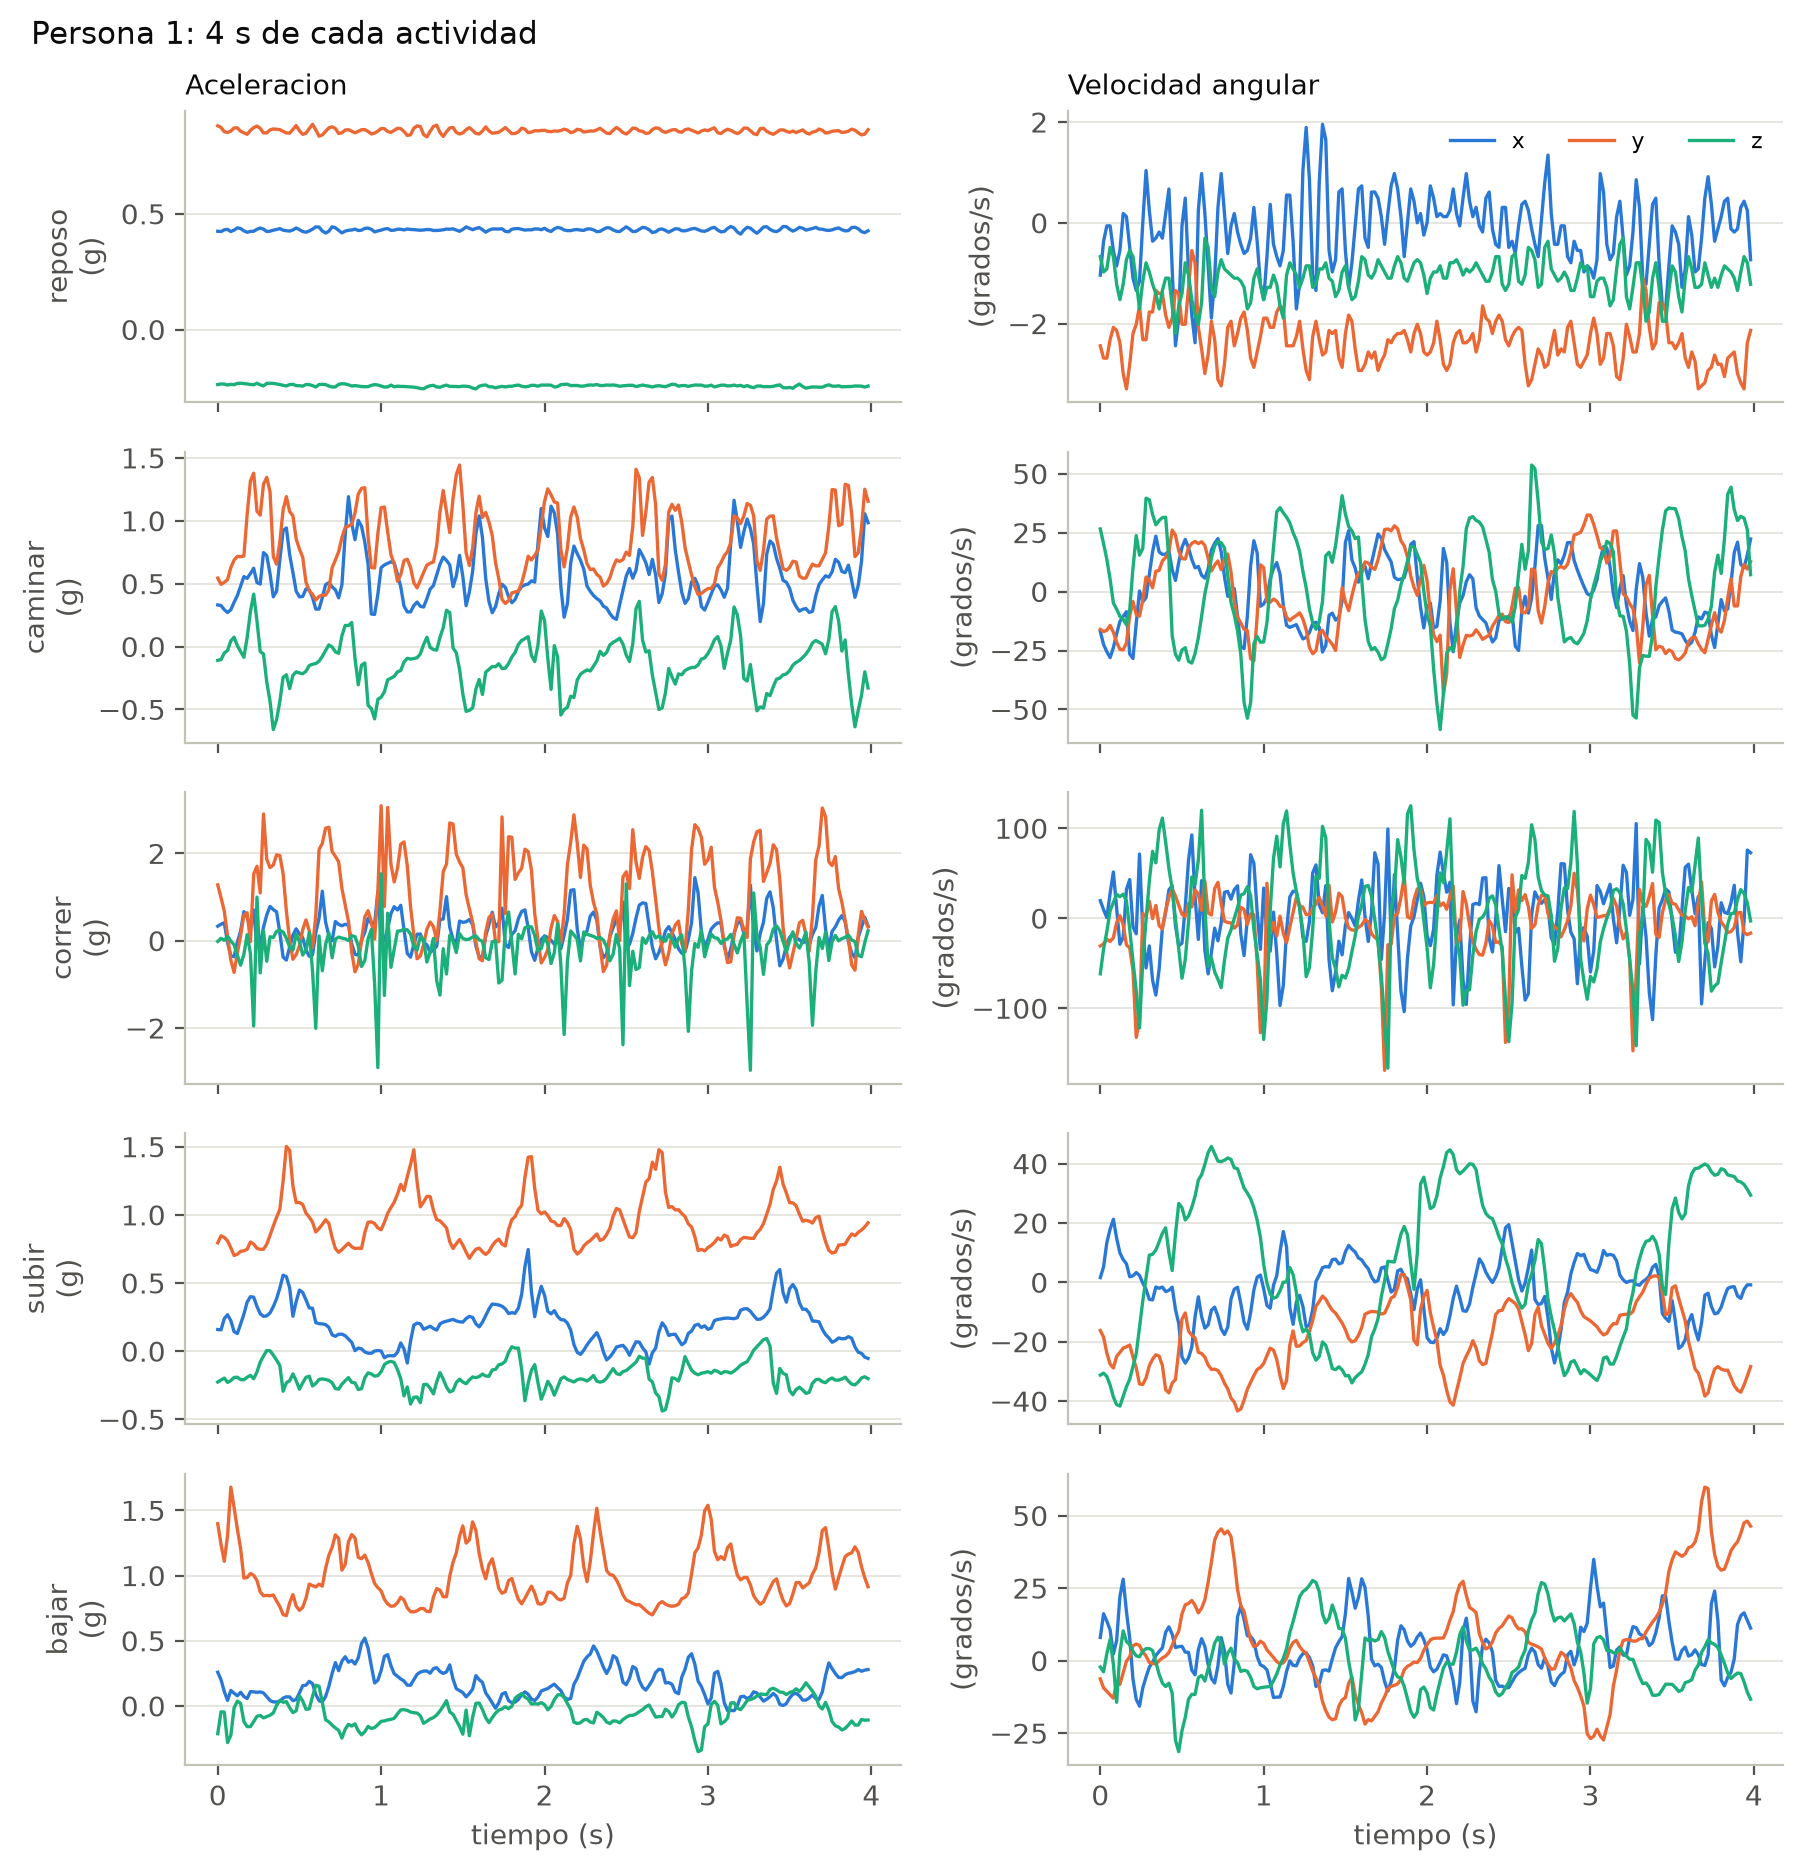
\includegraphics[width=0.92\linewidth]{1_fig_senales.png}
\caption{Señales de la persona~1 en 4~s del centro de cada sesión. En reposo, las tres componentes de la aceleración son constantes y distintas de cero porque son la gravedad proyectada según la inclinación de la placa.}
\label{fig:senales}
\end{figure}

\paragraph{Diferencias entre personas.}
Dos hallazgos condicionaron el diseño. El primero es que la inclinación de la placa cambió entre personas. En reposo, $a_x$ promedió 0.43~$g$ en la persona~1 y $-0.07~g$ en la persona~3. El segundo es que en las escaleras hubo un giro sostenido alrededor del eje vertical, por las vueltas en los descansos. Ese giro tuvo sentido opuesto en la persona~3 respecto a las otras dos, como muestra la figura~\ref{fig:giro}.

\begin{figure}[htbp]
\centering
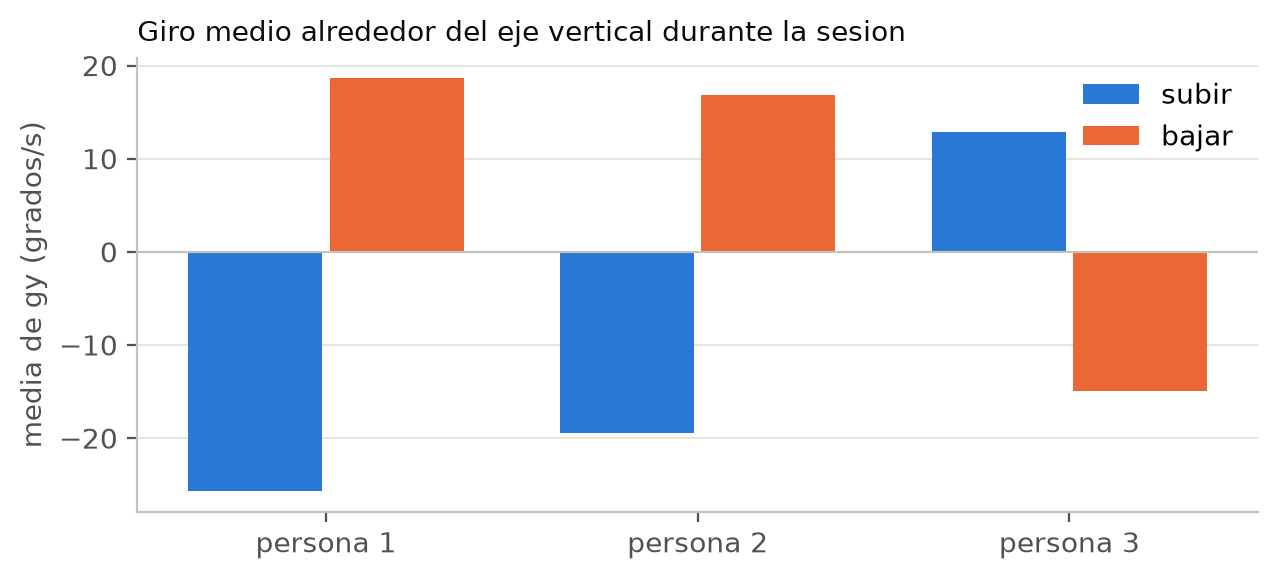
\includegraphics[width=0.62\linewidth]{1_fig_giro_escaleras.png}
\caption{Media de $g_y$, el giro alrededor del eje vertical, en las sesiones de escaleras.}
\label{fig:giro}
\end{figure}

\section{Preprocesamiento y protocolo de evaluación}\label{sec:prepro}

\paragraph{Ventanas.}
Se descarta 1~s al inicio y al final de cada sesión. Cada sesión se divide en ventanas de 100 muestras, es decir de 2~s, con un paso de 25 muestras. Ese paso equivale a 0.5~s y a un traslape de 75\,\%. La placa clasifica con el mismo paso.

\paragraph{Resta de la media por ventana.}
A cada canal se le resta su media dentro de la ventana. En el acelerómetro esa media es sobre todo la gravedad, que depende de cómo se colocó la placa. En el giróscopo es el giro sostenido más el sesgo. Después se normaliza cada canal con la media y la desviación del conjunto de entrenamiento. En el modelo final con acelerómetro, las desviaciones son 0.201, 0.450 y 0.229~$g$ en los ejes $x$, $y$ y $z$.

\paragraph{Partición.}
La evaluación deja una persona fuera, lo que se conoce como LOSO. Se entrena con dos personas y se prueba con todas las ventanas de la tercera, rotando las tres. Así ninguna ventana de una sesión de prueba aparece en el entrenamiento, como pide el enunciado. Para la detención temprana se usa como validación el último 20\,\% de cada sesión de entrenamiento. Ese tramo se ventanea por separado para que no comparta muestras con el entrenamiento. Cada pliegue usa 890 ventanas de entrenamiento, 200 de validación y 565 de prueba, y se repite con tres semillas.

\paragraph{Ablación.}
La figura~\ref{fig:ablacion} justifica las decisiones con el modelo de acelerómetro más giróscopo en FP32. Sin restar la media, la exactitud LOSO fue de 0.27. El modelo reconocía a las personas de entrenamiento por la inclinación de la placa, y en una persona nueva no acertó el reposo en ninguna de sus 1\,017 ventanas. Restar la media solo al giróscopo no ayudó, pues dio 0.29. Eso ubica el problema en la gravedad del acelerómetro. Restar la media en los seis canales subió la exactitud a 0.72 con una red de campo receptivo corto y a 0.77 con la red elegida, que se describe en la sección~\ref{sec:modelo}. Agregar copias con rotaciones 3D aleatorias de hasta 20~grados dio 0.78, casi lo mismo, por lo que no se usó.

\begin{figure}[htbp]
\centering
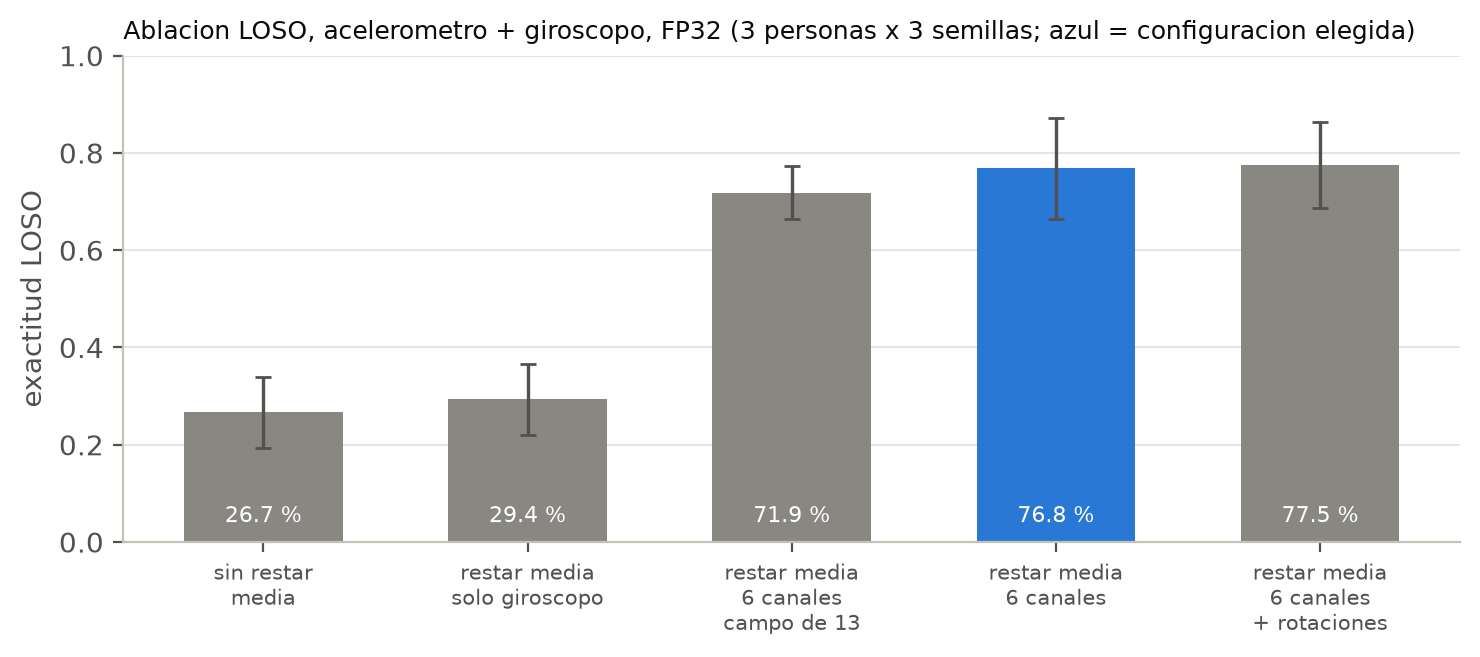
\includegraphics[width=0.85\linewidth]{2_fig_ablacion.png}
\caption{Ablación LOSO con la media y la desviación de 3 personas por 3 semillas, tomada de \texttt{2\_tab\_ablacion.csv}. «Campo de 13» es una red sin \emph{pooling} cuya última convolución ve 13 muestras.}
\label{fig:ablacion}
\end{figure}

\section{Modelo}\label{sec:modelo}

Es una red convolucional 1D, descrita en la tabla~\ref{tab:arq}. La última convolución ve 59 muestras, que equivalen a 1.2~s y cubren más de un ciclo de paso. Con dos convoluciones sin \emph{pooling} veía solo 13 muestras, es decir 0.26~s, y en esa versión caminar casi no se distinguía de las escaleras. El promedio global hace que la salida no dependa de en qué parte de la ventana cae cada paso.

Se entrena con Adam con una tasa de aprendizaje de 0.001, lotes de 32 y entropía cruzada. La detención temprana usa una paciencia de 10 épocas sobre la pérdida de validación y restaura los mejores pesos, con un máximo de 80 épocas. Los modelos finales se entrenaron con las tres personas. El de acelerómetro paró en 41 épocas y el de ambos sensores en 42, como muestra la figura~\ref{fig:entrenamiento}.

\begin{table}[htbp]
\centering\small
\begin{tabular}{llrr}
\toprule
Capa & Salida & Parámetros & MAC \\
\midrule
Conv1D, 16 filtros, $k$=5, $s$=2, ReLU & 48$\times$16 & 256 & 11\,520 \\
MaxPool, 2 & 24$\times$16 & 0 & 0 \\
Conv1D, 32 filtros, $k$=5, ReLU & 20$\times$32 & 2\,592 & 51\,200 \\
MaxPool, 2 & 10$\times$32 & 0 & 0 \\
Conv1D, 32 filtros, $k$=5, ReLU & 6$\times$32 & 5\,152 & 30\,720 \\
Promedio global & 32 & 0 & 0 \\
Dropout, 0.3 & 32 & 0 & 0 \\
Dense, 5 salidas, softmax & 5 & 165 & 160 \\
\midrule
Total con entrada de 100$\times$3 & & 8\,165 & 93\,600 \\
\bottomrule
\end{tabular}
\caption{Arquitectura del modelo con solo acelerómetro, tomada de \texttt{3\_tab\_arquitectura.csv}. Con acelerómetro más giróscopo la entrada es de 100$\times$6, con 8\,405 parámetros y 105\,120 MAC.}
\label{tab:arq}
\end{table}

\begin{figure}[htbp]
\centering
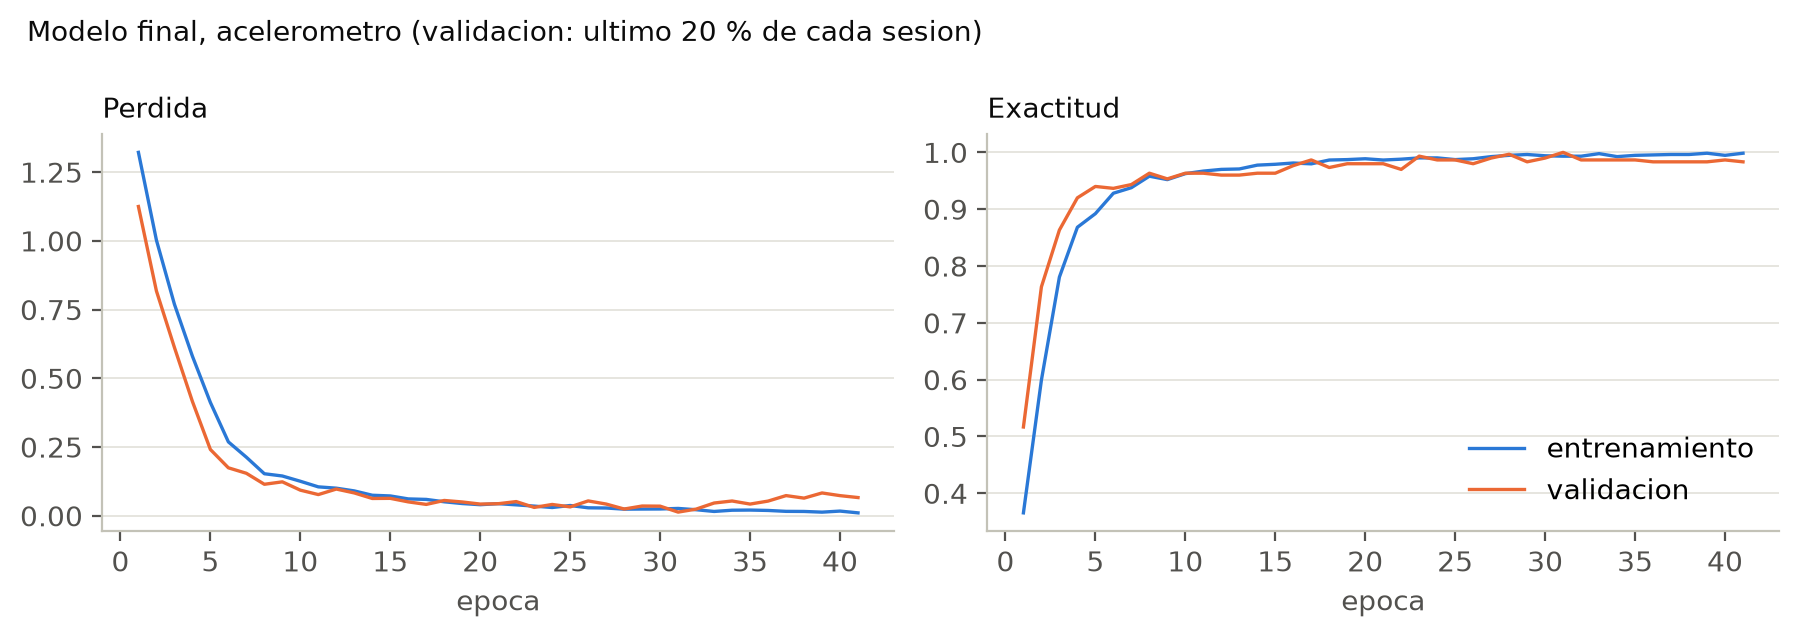
\includegraphics[width=0.85\linewidth]{3_fig_entrenamiento.png}
\caption{Entrenamiento del modelo final con acelerómetro. La validación es el último 20\,\% de las sesiones de las mismas personas, así que su exactitud de 1.00 es optimista y no mide la generalización.}
\label{fig:entrenamiento}
\end{figure}

\section{Cuantización a INT8}

Se usó cuantización entera completa con el conversor de TensorFlow~2.21. La entrada, la salida y los pesos quedan en int8 y los sesgos en int32. Las activaciones se calibran con 300 ventanas de entrenamiento. Los pesos de las convoluciones tienen una escala por filtro, que los kernels CMSIS-NN de la biblioteca \texttt{Chirale\_TensorFlowLite} 2.0.0 sí aplican. En cambio, su kernel \texttt{FULLY\_CONNECTED} int8 usa una sola escala por capa, como se encontró en el proyecto~1. Por eso la capa densa se cuantizó con una escala por capa.

La entrada quedó con escala 0.1022 y punto cero 23, así que representa de $-15.4$ a $10.6$ desviaciones estándar. Ese rango lo imponen las ventanas de correr. Las demás actividades quedan dentro de $\pm4.4$ y usan solo una fracción de los 256 niveles. La salida usa escala $1/256$ y punto cero $-128$, que es lo usual para probabilidades. Ambos modelos usan siete operadores y todos están soportados: \texttt{CONV\_2D}, \texttt{EXPAND\_DIMS}, \texttt{RESHAPE}, \texttt{MAX\_POOL\_2D}, \texttt{MEAN}, \texttt{FULLY\_CONNECTED} y \texttt{SOFTMAX}. Las convoluciones 1D aparecen como convoluciones 2D de altura 1.

\section{Implementación en el Arduino}

\begin{figure}[htbp]
\centering
\begin{tikzpicture}[
  bloque/.style={draw, rounded corners=2pt, align=center, font=\small, minimum height=1.1cm, text width=2.3cm},
  flecha/.style={-{Stealth[length=2.2mm]}, thick}]
\node[bloque] (imu) {IMU LSM9DS1\\lectura a 50~Hz};
\node[bloque, right=0.55cm of imu] (buf) {Buffer circular\\de 100 muestras};
\node[bloque, right=0.55cm of buf] (pre) {Restar media,\\$(x-\mu)/\sigma$\\y cuantizar};
\node[bloque, right=0.55cm of pre] (red) {CNN INT8\\TFLite Micro};
\node[bloque, below=0.8cm of red] (suav) {Promedio de\\3 ventanas};
\node[bloque, left=0.55cm of suav] (serie) {Monitor Serie\\cada 0.5~s};
\draw[flecha] (imu) -- (buf);
\draw[flecha] (buf) -- (pre);
\draw[flecha] (pre) -- (red);
\draw[flecha] (red) -- (suav);
\draw[flecha] (suav) -- (serie);
\end{tikzpicture}
\caption{Flujo en la placa. Cada 25 muestras nuevas se clasifica la última ventana de 2~s.}
\label{fig:flujo}
\end{figure}

La figura~\ref{fig:flujo} muestra el flujo del programa. Lee la IMU cada 20~ms con un temporizador basado en \texttt{micros()} y guarda las seis columnas crudas en un buffer circular de 100 muestras. Cada 25 muestras nuevas ordena la ventana y le resta la media, que acumula en doble precisión. Luego normaliza con las constantes del entrenamiento y cuantiza la entrada con $q = \mathrm{round}(x/s) + z$, saturada a $[-128, 127]$. Después ejecuta el modelo y descuantiza las probabilidades.

En cada predicción imprime la clase con mayor probabilidad promedio en las tres últimas ventanas, que abarcan 1.5~s de historia. También imprime la clase de la ventana actual, el tiempo de inferencia y cuántas lecturas se retrasaron más de un periodo. Todo se muestra en el Monitor Serie.

El programa incluye una autoprueba para verificar que el preprocesamiento en C coincide con el de Python. Al arrancar clasifica cinco ventanas crudas del conjunto de validación, una por clase y de distintas personas. Luego compara sus probabilidades con las que dio TensorFlow Lite en Python. Después mide 100 inferencias con \texttt{micros()} alrededor de \texttt{Invoke()} y mide por separado el tiempo del preprocesamiento.

Se generaron cuatro programas. Dos usan solo el acelerómetro, uno en INT8 y otro en FP32. El de INT8 es el de la demostración. Los otros dos usan acelerómetro más giróscopo, también en INT8 y en FP32. Todos usan \texttt{MicroMutableOpResolver<7>} con los operadores listados y una \emph{tensor arena} de 32~KB. Se compilaron con \texttt{arduino-cli}~1.5.1 y el paquete Arduino Mbed OS Nano Boards~4.6.0. La tabla~\ref{tab:placa} resume la memoria que ocupan.

\section{Evaluación experimental}

\subsection{Exactitud y matriz de confusión}

Con solo el acelerómetro, la exactitud LOSO fue de 0.831. Probando con la persona~1 fue de 0.918, con la persona~2 de 0.855 y con la persona~3 de 0.720, como muestra la tabla~\ref{tab:loso}. Promediar tres ventanas consecutivas, como hace la placa, la sube a 0.841. El F1 macro, calculado sobre la matriz sumada de los tres pliegues y las tres semillas, fue de 0.831.

Reposo y correr se reconocen casi siempre, con F1 de 1.00 y 0.99, según la tabla~\ref{tab:clases}. Los errores se concentran en las actividades de marcha. Caminar se reconoce en el 57\,\% de sus ventanas y se confunde sobre todo con bajar escaleras, en un 28\,\%. Subir escaleras se confunde con bajar en el 32\,\% de sus ventanas. Por eso bajar escaleras tiene una exhaustividad alta de 0.93 pero una precisión baja de 0.60. Las otras dos clases de marcha caen en ella.

\begin{table}[htbp]
\centering\small
\begin{tabular}{lcccc}
\toprule
Persona de prueba & FP32 & FP32, promedio de 3 & INT8 & INT8, promedio de 3 \\
\midrule
1 & 0.918 $\pm$ 0.041 & 0.936 & 0.912 & 0.932 \\
2 & 0.855 $\pm$ 0.017 & 0.853 & 0.866 & 0.853 \\
3 & 0.720 $\pm$ 0.006 & 0.735 & 0.720 & 0.735 \\
\midrule
Las tres & 0.831 $\pm$ 0.086 & 0.841 & 0.832 & 0.840 \\
\bottomrule
\end{tabular}
\caption{Exactitud LOSO con solo acelerómetro. Se muestra la media y la desviación sobre 3 semillas, tomadas de \texttt{4\_tab\_loso.csv}.}
\label{tab:loso}
\end{table}

\begin{table}[htbp]
\centering\small
\begin{tabular}{lcccr}
\toprule
Clase & Precisión & Exhaustividad & F1 & Ventanas \\
\midrule
Reposo & 0.999 & 1.000 & 1.000 & 1\,017 \\
Caminar & 0.972 & 0.570 & 0.719 & 1\,017 \\
Correr & 0.995 & 0.982 & 0.989 & 1\,017 \\
Subir escaleras & 0.772 & 0.672 & 0.718 & 1\,017 \\
Bajar escaleras & 0.599 & 0.931 & 0.729 & 1\,017 \\
\midrule
Macro & 0.867 & 0.831 & 0.831 & 5\,085 \\
\bottomrule
\end{tabular}
\caption{Métricas por clase con solo acelerómetro en FP32, sumando los tres pliegues y las tres semillas. Datos de \texttt{4\_tab\_por\_clase.csv}.}
\label{tab:clases}
\end{table}

\begin{figure}[htbp]
\centering
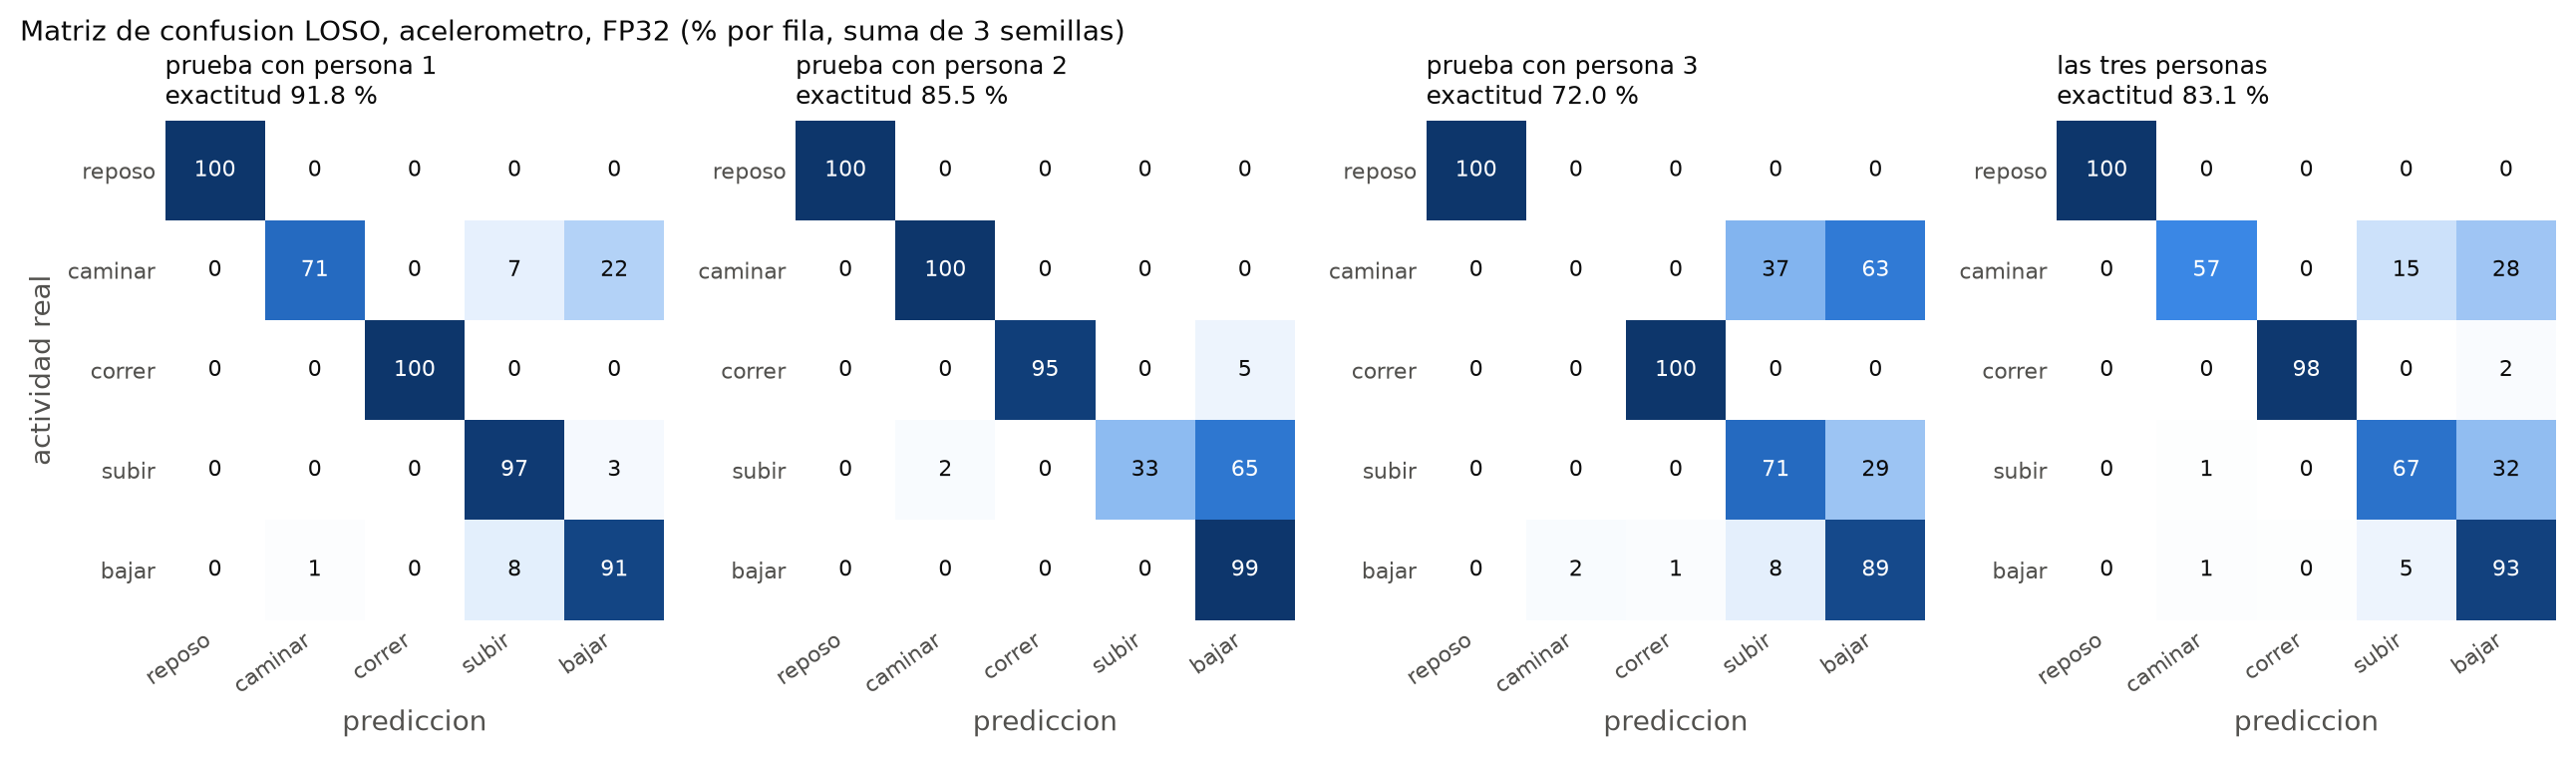
\includegraphics[width=\linewidth]{4_fig_confusion.png}
\caption{Matrices de confusión LOSO con solo acelerómetro en FP32. Cada celda es el porcentaje de su fila.}
\label{fig:confusion}
\end{figure}

\subsection{Acelerómetro frente a acelerómetro más giróscopo}

Agregar el giróscopo empeoró la generalización. La exactitud bajó de 0.831 a 0.768 y el F1 empeoró en todas las clases salvo reposo, como muestran la tabla~\ref{tab:sensores} y la figura~\ref{fig:sensores}. La exactitud bajó con las tres personas de prueba, sobre todo con la persona~2, donde pasó de 0.855 a 0.745. También varió más entre semillas. Con la persona~2, su desviación fue de 0.086 contra 0.017 del acelerómetro solo.

Con solo dos personas de entrenamiento, los tres canales adicionales parecen dar al modelo más formas de ajustarse a particularidades de esas personas que información que se transfiera. Es una hipótesis que no está verificada. Sí se probó y se descartó otra explicación, el sentido de giro en los descansos de la escalera. En una exploración preliminar con 2 semillas, quitar $g_y$ o aumentar los datos con su versión en espejo dio 0.75, frente a 0.78 sin esos cambios.

\begin{table}[htbp]
\centering\small
\begin{tabular}{lcccccccc}
\toprule
Sensores & Canales & Exactitud & F1 macro & \multicolumn{5}{c}{F1 por clase} \\
\cmidrule(lr){5-9}
 & & & & Rep. & Cam. & Corr. & Subir & Bajar \\
\midrule
Acelerómetro & 3 & 0.831 & 0.831 & 1.00 & 0.72 & 0.99 & 0.72 & 0.73 \\
Acel. + giróscopo & 6 & 0.768 & 0.768 & 1.00 & 0.57 & 0.91 & 0.67 & 0.68 \\
\bottomrule
\end{tabular}
\caption{Comparación de sensores con LOSO en FP32, tomada de \texttt{5\_tab\_sensores.csv}.}
\label{tab:sensores}
\end{table}

\begin{figure}[htbp]
\centering
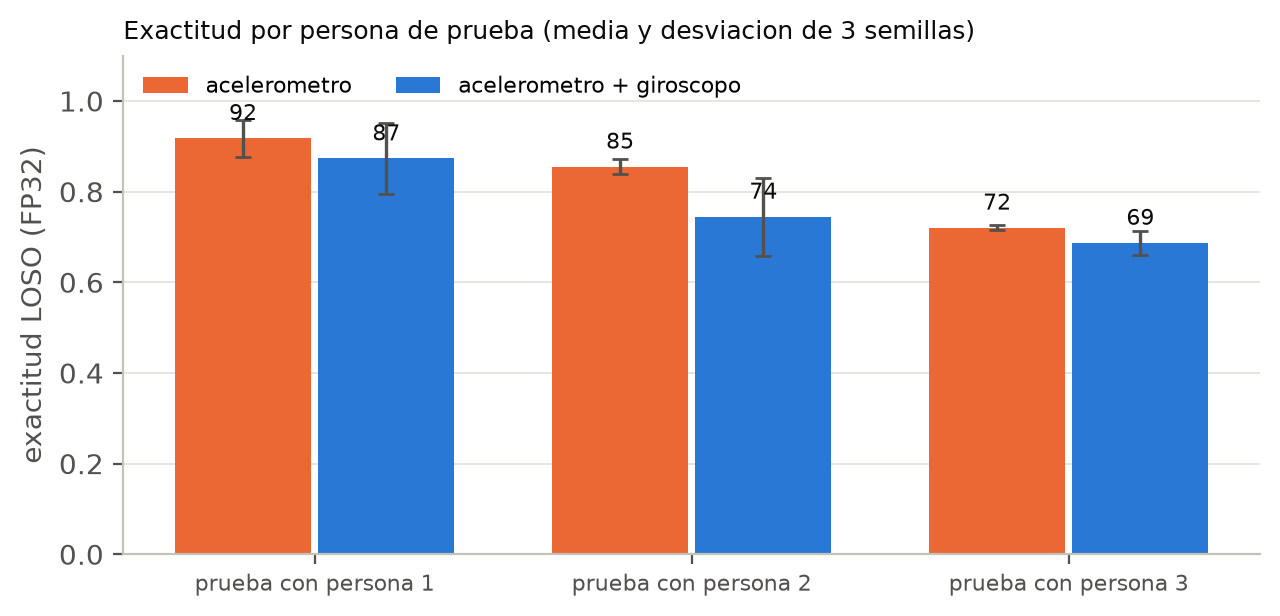
\includegraphics[width=0.7\linewidth]{5_fig_sensores.png}\\[4pt]
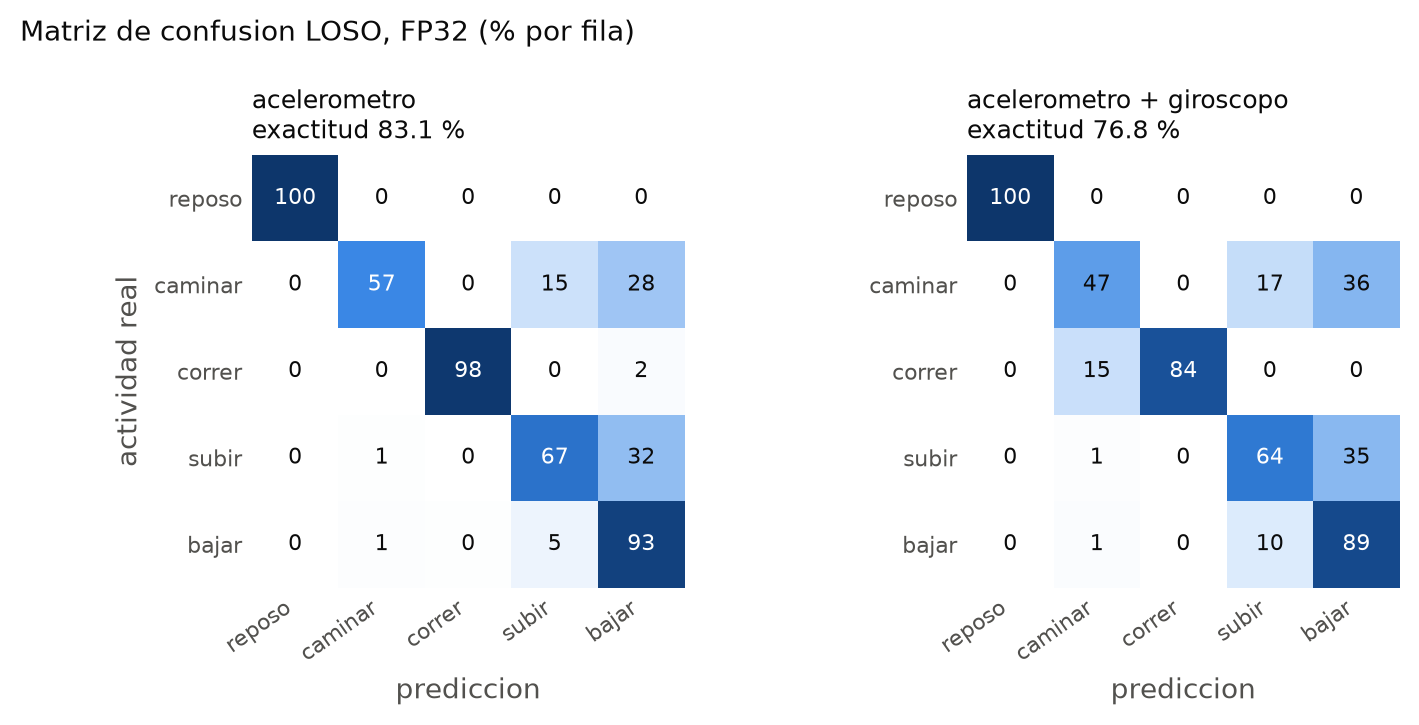
\includegraphics[width=0.75\linewidth]{5_fig_confusion_sensores.png}
\caption{Arriba, la exactitud por persona de prueba. Abajo, las matrices de confusión de ambos modelos.}
\label{fig:sensores}
\end{figure}

\subsection{Modelo original FP32 frente al cuantizado INT8}

En cada pliegue LOSO se cuantizó el modelo entrenado y se evaluó con la misma persona de prueba. La exactitud no cambió de forma apreciable. Con acelerómetro pasó de 0.831 a 0.832 y con ambos sensores de 0.768 a 0.767. Las predicciones INT8 coinciden con las FP32 en el 98.6\,\% y el 98.8\,\% de las ventanas, respectivamente, como muestra la figura~\ref{fig:cuant}.

El archivo del modelo se redujo 55\,\%. La Flash del programa bajó unos 21~KB, lo mismo que se redujo el modelo. La RAM estática es igual en ambos porque la arena reservada es la misma, como se ve en la tabla~\ref{tab:placa}.

\begin{figure}[htbp]
\centering
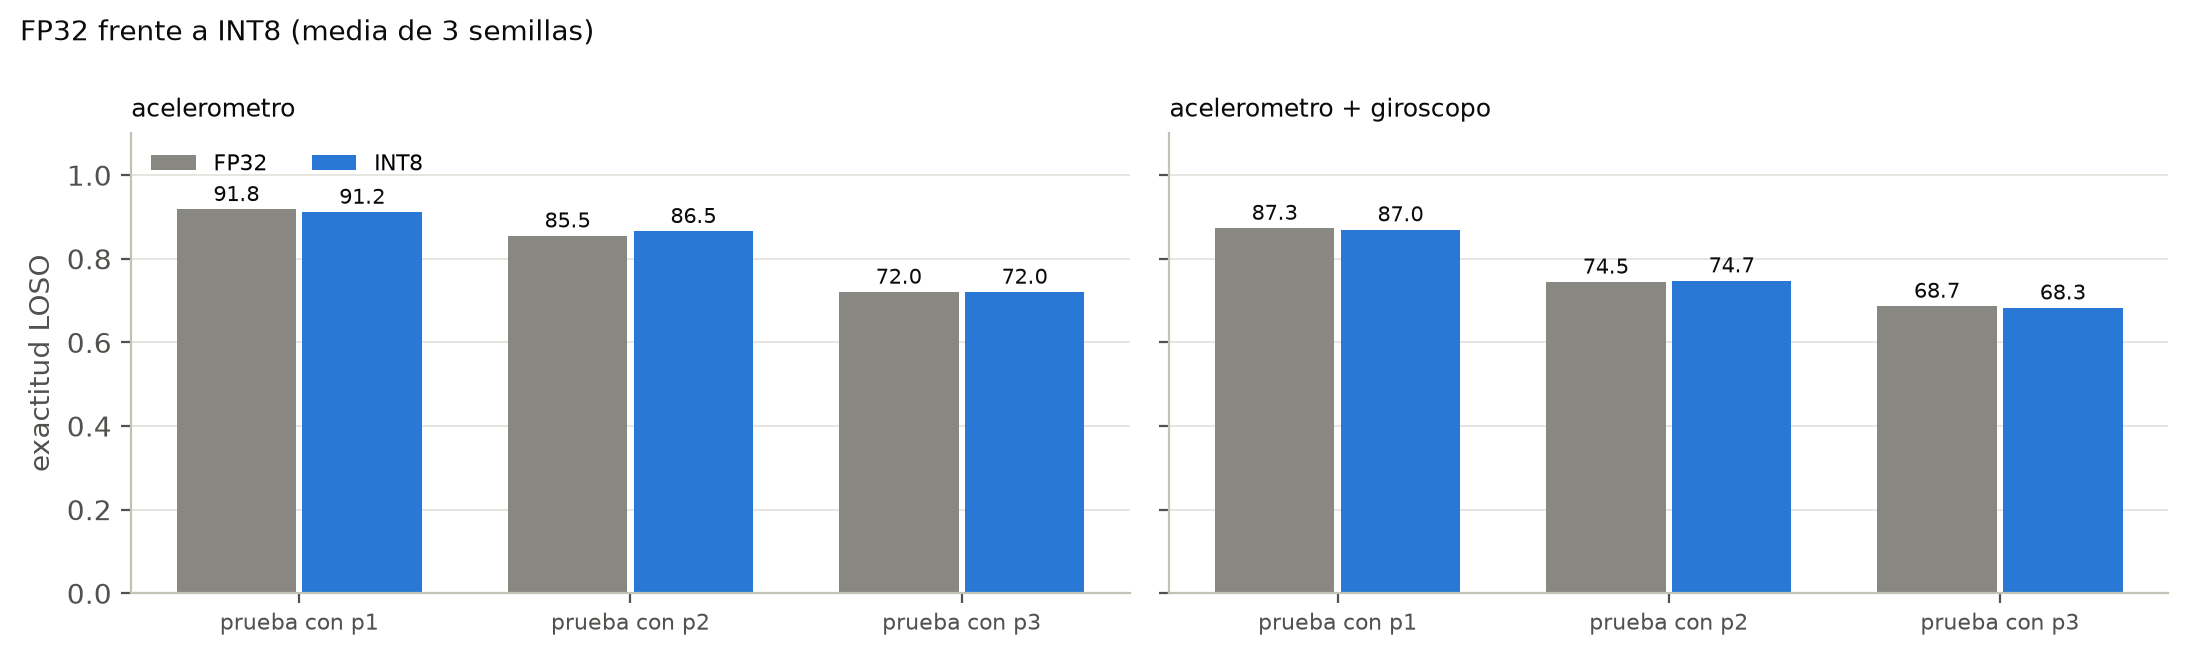
\includegraphics[width=0.95\linewidth]{6_fig_cuantizacion.png}
\caption{Exactitud LOSO de FP32 frente a INT8 por persona de prueba, como media de 3 semillas.}
\label{fig:cuant}
\end{figure}

\begin{table}[htbp]
\centering\small
\begin{tabular}{lrrrrrr}
\toprule
Programa & Modelo (B) & Flash (B) & RAM est. (B) & Arena usada (B) & Latencia ($\mu$s) & Autoprueba \\
\midrule
Acel., INT8 & 17\,728 & 193\,176 & 84\,656 & \pendiente{} & \pendiente{} & \pendiente{} \\
Acel., FP32 & 39\,156 & 214\,600 & 84\,656 & \pendiente{} & \pendiente{} & \pendiente{} \\
Acel. + gir., INT8 & 18\,200 & 193\,696 & 84\,656 & \pendiente{} & \pendiente{} & \pendiente{} \\
Acel. + gir., FP32 & 40\,376 & 215\,872 & 84\,656 & \pendiente{} & \pendiente{} & \pendiente{} \\
\bottomrule
\end{tabular}
\caption{Memoria y latencia en la placa, tomadas de \texttt{7\_tab\_placa.csv}. La Flash y la RAM estática salen de la compilación, de 983\,040 y 262\,144~B disponibles. La RAM estática incluye la arena de 32~KB. La latencia es el promedio de 100 inferencias.}
\label{tab:placa}
\end{table}

\section{Demostración funcional}

La demostración usa el programa con solo acelerómetro en INT8. \pendiente{describir la sesión: quién hizo las actividades, dónde y con qué colocación, el resultado de la autoprueba, donde se espera coinciden~=~5/5, la captura del Monitor Serie, el valor de \texttt{muestras\_tarde}, las observaciones por actividad y los nombres de los videos en el zip}.

\section{Discusión y limitaciones}

\begin{itemize}
\item Con tres personas y una sesión por actividad, la estimación es variable. La exactitud va de 0.72 a 0.92 según la persona de prueba, y la persona~3 es la más difícil para ambos modelos.
\item La exactitud de validación de los modelos finales fue de 1.00, pero se mide con ventanas de las mismas sesiones y personas. No indica generalización. La cifra representativa es la de LOSO.
\item El preprocesamiento y la arquitectura se eligieron viendo los resultados LOSO, que son la única evaluación posible con tres personas. Por eso esas cifras pueden ser algo optimistas. La ablación completa está en la figura~\ref{fig:ablacion}.
\item Restar la media elimina la orientación estática, pero no las diferencias de orientación en la parte dinámica de la señal. Una colocación muy distinta a la de la captura puede degradar el resultado.
\item Las confusiones entre caminar, subir y bajar escaleras dominan el error. Los siguientes pasos naturales son agregar más personas y sesiones o probar ventanas más largas.
\end{itemize}

\section{Conclusiones}

\pendiente{revisar al tener las mediciones de la placa}. Restar la media de cada ventana fue la decisión más importante. Sin ella el modelo memoriza cómo cada persona llevó la placa y falla con personas nuevas, con una exactitud de 0.27 contra 0.77. La segunda decisión importante fue que la red viera al menos un ciclo de paso. El acelerómetro solo generalizó mejor que junto con el giróscopo, con 0.831 contra 0.768. La cuantización INT8 redujo el modelo a menos de la mitad sin perder exactitud. Falta medir en la placa si también reduce la latencia.

\section{Archivos entregados}

\begin{itemize}
\item \texttt{Proyecto\_3.py} hace el preprocesamiento, la evaluación LOSO, la ablación, el entrenamiento final, la cuantización y la generación de los programas.
\item \texttt{compilar\_sketches.py} compila los programas sin la placa y anota su memoria. \texttt{requirements.txt} lista las bibliotecas de Python.
\item \texttt{datos/} contiene los tres archivos CSV del conjunto de datos.
\item \texttt{resultados/} contiene las tablas, las figuras, los modelos \texttt{.keras} y \texttt{.tflite} y la salida de la compilación.
\item \texttt{arduino/} contiene los cuatro programas, cada uno con su \texttt{.ino}, \texttt{model.h} y \texttt{har\_config.h}, y las instrucciones.
\item \pendiente{videos de la demostración y capturas del Monitor Serie}.
\end{itemize}

En Python se usaron Python 3.13.1, TensorFlow 2.21.0, Keras 3.15.1, NumPy 2.5.5 y pandas 3.1.1. Para la placa se usaron Arduino Mbed OS Nano Boards 4.6.0, \texttt{Chirale\_TensorFlowLite} 2.0.0 y \texttt{Arduino\_LSM9DS1} 1.1.1.

\end{document}
